\documentclass[parskip=full]{scrartcl}

\usepackage[utf8]{inputenc}			% Umlaute, Sonderzeichen
\usepackage[ngerman]{babel}			% deutsche Sprache
\usepackage{enumitem}				% Listen
\usepackage{graphicx}				% Grafiken
\usepackage{hyperref}				% Hyperlinks
\usepackage[nonumberlist]{glossaries}		% Glossar
\usepackage{amsmath}
\usepackage{pdfpages}				% PDF einbinden


\makenoidxglossaries



\subject{Benutzerhandbuch}
\title{Handbuch zur Benutzung der Anwendung "FreeJDAQ"}
\subtitle{Version 1.0.0}
\author{David Gawron \and Stefan Geretschläger \and Leon Huck \and Jan Küblbeck \and Linus Ruhnke}
\date{\today}


\begin{document}

\maketitle

\clearpage
\tableofcontents 					% generate pdf twice to update

\section{Einleitung}

\section{Beschreibung der graphischen Benutzeroberfläche}

\begin{figure}[htbp]
    \begin{center}
        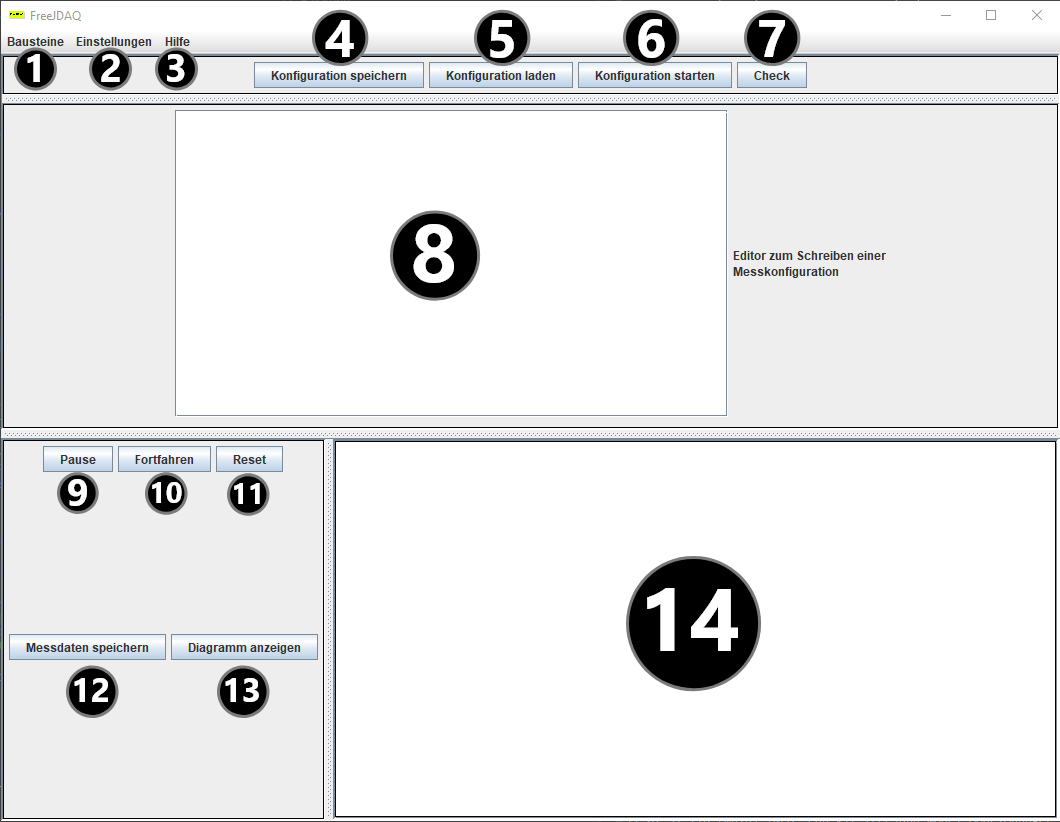
\includegraphics[width = 10cm]{Grafiken/Uebersicht_GUI_Mit_Nummern.png}
        \caption{Die Übersicht über die grafische Benutzeroberfläche von FreeJDAQ. Die Nummern verweißen auf die genauen Beschreibungen, die weiter unten zu finden sind.}
        \label{Uebersicht_GUI_Mit_Nummern}
    \end{center}
\end{figure}

\begin{enumerate}
    \item Bausteine
    
    \item Einstellungen
\end{enumerate}

\begin{flushleft}
    
\includegraphics[width = 2cm]{Grafiken/1-Bausteine.png}
\end{flushleft}

\begin{flushleft}
    
\includegraphics[width = 2cm]{Grafiken/2-Einstellungen.png}
\end{flushleft}

\begin{flushleft}
    
\includegraphics[width = 2cm]{Grafiken/3-Hilfe.png}
\end{flushleft}

\begin{flushleft}
    
\includegraphics[width = 2cm]{Grafiken/4-Konfiguration_speichern.png}
\end{flushleft}

\begin{flushleft}
    
\includegraphics[width = 2cm]{Grafiken/5-Konfiguration_laden.png}
\end{flushleft}

\begin{flushleft}
    
\includegraphics[width = 2cm]{Grafiken/6-Konfiguration_starten.png}
\end{flushleft}

\begin{flushleft}
    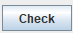
\includegraphics[width = 2cm]{Grafiken/7-Check.png}
\end{flushleft}

\begin{flushleft}
    
\includegraphics[width = 2cm]{Grafiken/8-Editor.png}
\end{flushleft}

\begin{flushleft}
    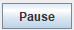
\includegraphics[width = 2cm]{Grafiken/9-Pause.png}
\end{flushleft}

\begin{flushleft}
    
\includegraphics[width = 2cm]{Grafiken/10-Fortfahren.png}
\end{flushleft}

\begin{flushleft}
    
\includegraphics[width = 2cm]{Grafiken/11-Reset.png}
\end{flushleft}

\begin{flushleft}
    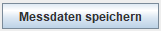
\includegraphics[width = 2cm]{Grafiken/12-Messdaten_speichern.png}
\end{flushleft}

\begin{flushleft}
    
\includegraphics[width = 2cm]{Grafiken/13-Diagramm_anzeigen.png}
\end{flushleft}

\begin{flushleft}
    
\includegraphics[width = 2cm]{Grafiken/14-Datenanzeige.png}
\end{flushleft}

\section{Beschreibung der Messkonfigurationssprache}


Im Folgenden Abschnitt wird erklärt, wie man eine Messkonfiguration erstellt und welche syntaktischen Regeln dabei eingehalten werden müssen.  

Eine Messkonfiguration besteht aus 3 zusammenhängenden Teilen., den Bausteinen, den Ein- und Ausgängen der Bausteine und den Verbindungen zwischen Aus- und Eingängen.  

\subsection{Bausteine}

Bausteine bezeichnen einen Knoten für die Datenverarbeitung. Ein Baustein kann 
Sensor, Transformation oder Transformation sein. werden der Messkonfiguration über ihren Namen hinzugefügt. Der Name lässt sich über das Systemmenü „Bausteine“ herausfinden.   
Das Format, in welchem die Bausteine besteht aus der Deklaration für die Bausteine benötigt das Schlüsselwort „blocks:“ Und die Bausteine werden wie folgend deklariert: 

\begin{itemize}

\item[ ] \textbf{blocks: [Baustein1, Baustein2, Baustein3]}

\end{itemize}

\subsection{Ein- und Ausgänge}

Ein- und Ausgänge repräsentieren Schnittstellen für die Verbindung von 2  
Bausteinen. Die Anzahl der Ein- und Ausgänge der Bausteine ist vordefiniert und kann unter „Bausteine -> Bearbeiten“ eingesehen werden. Daher muss die Anzahl der Ein- und Ausgänge in der Messkonfiguration dieser Anzahl entsprechen. Die Namen sind frei wählbar, aber einen eindeutigen und aussagekräftigen vereinfacht das Schreiben der Konfiguration.  
Das Format, in welchem die Ein- und Ausgänge deklariert werden besteht aus dem einem Schlüsselwort und der nachfolgenden Deklaration der Ein- und Ausgänge für jeden Baustein individuell. Das Schlüsselwort ist frei wählbar, jedoch muss die Reihenfolge der Deklaration der Reihenfolge der Baustein-Deklaration entsprechen:  

\begin{itemize}

\item[ ] \textbf{channelListBlock1: [B1out1, B1out2]}
\item[ ] \textbf{channelListBlock2: [T1in, T1out]}
\item[ ] \textbf{channelListBlock3: [R1in1, R1in2]} 

\end{itemize}

\subsection{Verbindungen}

Über Verbindungen zwischen Ein- und Ausgängen der Bausteine wird ein Datenflussmodel erzeugt, über welches die Messdaten laufen.  Eine Verbindung besteht immer zwischen einem Ausgang und einem Eingang, also einem Tupel aus Ausgang und Eingang.   
Das Schlüsselwort für die Verbindungen ist „configuration:“ und die Verbindungen werden wie folgend deklariert:  

\begin{itemize}

\item[ ] \textbf{configuration: [[B1out1, R1in1], [B1out2, T1in], [T1out, R1in2]]}

\end{itemize}

Ein Beispiel für eine solche Konfiguration ist die folgende, welche so in dem Konfigurationsfeld anzeigt werden sollte:

\begin{figure}[htbp]
    \begin{center}
        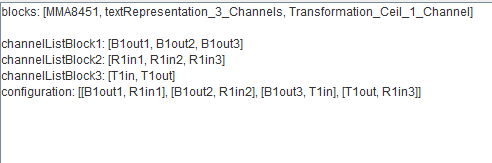
\includegraphics[width = 10cm]{Grafiken/KonfigBsp.png}
        \caption{Beispiel Konfiguration im Konfigurationsfeld}
        \label{KonfigBsp}
    \end{center}
\end{figure}



\section{Umgang mit dem Raspberry Pi}

\section{Fehlermeldungen}

\section{Limitierung der Anwendung}


\printnoidxglossaries				% generate pdf twice when adding new entries

\end{document}\grid
